\documentclass{article}
\usepackage{graphicx}
\usepackage{amsmath}
\usepackage{amsfonts}
\usepackage{graphicx}
\usepackage{hyperref}

\begin{document}

\title{QDN Network For Maze Solving}
\author{Axel Ind (\textit{4563539}), Fernando Cristiani \textit{(4527671)}}

\maketitle

\begin{abstract}
This document details work to create and evaluate a convolutional neural network that solves mazes with a partially observable environment using reinforcement learning. Training is conducted via bounded exploration of the environment. The network architecture consisted of 2 convolutional layers, each followed by a pooling layer and a single fully connected softmax output layer. Training  loss of $\approx 0.003$ is achieved for history $\geq 4$. Testing accuracy of $100\%$ is achieved for steps$>8000$.
\end{abstract}

\section{Dataset}
\subsection{Data Format}
Each input consists of 3-dimensional numeric input of depth $d$. The $25\times 25\times d$ matrix provides a instantaneous grayscale representation of the current state of the agent in the maze, and the same information for each of its last $d-1$ states. Individual values in the matrix range from $0$ to $255$ and are used to represent cell occupation.
\subsection{Data Generation}
Data is generated and integrated into the neural network after each action taken by the agent.

\section{Network Architecture}
\subsection{Inputs}
\textbf{Stochastic Gradient Descent}: $25 \times 25 \times d \times n$ (where $d$ is the history length, $n$ is the batch size).

\subsection{Outputs}
$Y=(y_0, y_1, y_2, y_{3}, y_{4})$

\noindent
Each class corresponds to a classification of: $(0,4) \in \mathbb{Z} $.

\noindent
More precisely the actions are mapped as follows:

\noindent
\begin{tabular}{ |c|c|c| } 
 \hline
 \textbf{Action} & \textbf{Agent Motion} \\ 
 0 & Do nothing \\ 
 1 & Up \\ 
 2 & Down\\
 3 & Left \\ 
 4 & Right\\
 \hline
\end{tabular}

\section{Training}

\subsection{Propagation}
All training results are achieved using the AdamOptimizer to update weights.

\subsection{Testing Hyperparameters}
\begin{itemize}
\item \textbf{Network architecture}: $\textrm{Input}-\{\textrm{Conv-Relu-Pool}\}^2-\textrm{FullyConnectedLayer-Softmax}$
\item \textbf{NumFilters}: $32^{|1|},32^{|2|}$
\item \textbf{KernelSize}: $5\times 5$
\item \textbf{BatchSize}: $32$
\item \textbf{Stride}: 2
\item \textbf{DiscountFactor}: $0.8$
\end{itemize}

\subsection*{Testing Architecture}




\begin{tabular}{ |c|c|c| } 
 \hline
 CPU & i7-6700HQ \\ 
 GPU & GTX970 (6GB) \\ 
 RAM & 16GB \\ 
 Hard Disk & SSD\\
 \hline
\end{tabular}

\newpage

\section{Questions}
\subsection{Update rule for Q-Function}
\begin{equation}
\label{eq:q}
Q(i,u)=(1-\alpha)Q(i,u)+\alpha \left( r(i,u) + (\gamma=0.5) {max}_{u' \in U_j}  Q(j,u')-Q(j,u')\right)
\end{equation}

where $i$ is the intitial state, $j$ is the successor state, $\alpha$ is the learning rate, $u$ is the action taken from $i$, $U_j$ is the set of applicable operators from state $j$ and $\gamma$ is the learning rate. 


\subsection{Transitions to Absorbing Goal State}
\begin{itemize}
\item Equation~\ref{eq:q} accurately describes the update procedure for a transition to an absorbing goal state. However, the reward for entering the goal state could be set \textit{a priori} to allow the $Q$-function to update accurately.
\end{itemize}

\subsection{Transitions from Absorbing Goal State}
\begin{itemize}
\item The Q-value of transitions from absorbing goal states should not change, therefore a check should be added to Equation~\ref{eq:q}. This would require a lookup table of goal states.
\item Option 1: Prevent any actions from being valid in the goal state. (As is Figure~\ref{fig:qFunctionTable}).
\item Option 2: Set the cost of any action from a goal state (except ``Do Nothing'') to $\infty$.
\item Option 3: End the simulation when the goal is reached\footnote{This is the method applied in the implementation this paper describes}.
\end{itemize}

\subsection{Q-Function Example}
\subsubsection*{Changed Q-Values}
\[Q((0,0),u=d), [Q((1,0),u=r), [Q((1,1),u=u),[Q((1,1),u=r), [Q((1,2),u=u)\]

\begin{figure}[ht!]
\centering
  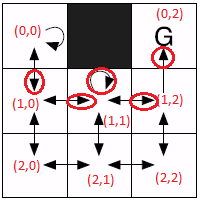
\includegraphics[width=0.4\linewidth]{qfunction}
  \caption{Figure showing the changed Q-functions in the toy example.}
  \label{fig:qFunctionTable}
\end{figure}
\subsubsection*{Improved Q-Values}
\begin{enumerate}
\item \[Q((0,0),u=d)=-1+0.5(0)=-1\]
\item \[Q((1,0),u=r)=-1+0.5(0)=-1\]
\item \[Q((1,1),u=u)=-1+0.5(0)=-1\]
\item \[Q((1,1),u=r)=-1+0.5(0)=-1\]
\item \[Q((1,2),u=u)=-1+0.5(0)=-1\]
\item All other $Q$ values are $0$.
\end{enumerate}




%--------------------------------------------------------------

\section{Results}
\subsection{Loss}
The AdamOptimizer was used to minimize the loss function described in \textit{q\_loss.Q\_loss()}. Loss values show a weakly-logarithmic decrease (Figure~\ref{fig:loss}).
\begin{figure}[ht!]
\centering
  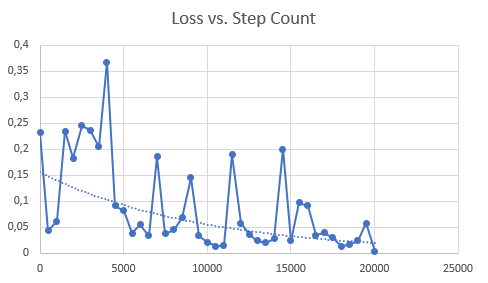
\includegraphics[width=0.8\linewidth]{loss}
  \caption{Graph showing the loss values (500-step intervals) achieved by the QDN.}
  \label{fig:loss}
\end{figure}

\subsubsection*{Notes on Loss}
\textbf{Normalization}: Normalising $Q$-Values prevented gradient divergence.

\subsection{Goal-Finding Accuracy}
\begin{itemize}
\item \textbf{Learning Rate}: $0.0005$
\item \textbf{Dropout}: $0.4$
\item \textbf{Alpha} (exploration): $0.3$
\end{itemize}

The agent is able to accurately reach the goal $100\%$ of the time after 2000th step for the small training map (Figure~\ref{fig:accuracy}).

\begin{figure}[ht!]
\centering
  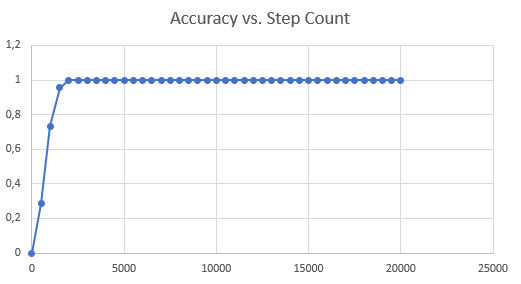
\includegraphics[width=0.8\linewidth]{accuracy}
  \caption{Graph showing the accuracy values (500-step intervals) achieved by the QDN.}
  \label{fig:accuracy}
\end{figure}

\subsection{Changed Target}
A trained agent adapts to the new target very quickly (Figure~\ref{fig:accuracy_new}) and after $1500$ training steps is able to reach the goal with $100\%$ accuracy.
\begin{figure}[ht!]
\centering
  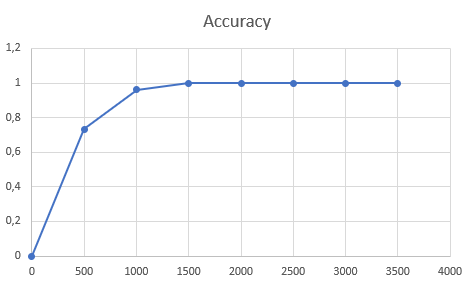
\includegraphics[width=0.8\linewidth]{accuracy_new}
  \caption{Graph showing the accuracy values (500-step intervals) achieved by the trained QDN with a new target.}
  \label{fig:accuracy_new}
\end{figure}
\subsection{Changed Map}
For the purposes of this experiment, the trained agent was made to train on an unseen map environment. It quickly adapted to the new map and, after $1500$ training steps, was able to reach the new goal with $100\%$ accuracy (Figure~\ref{fig:accuracy_T}).

\begin{figure}[ht!]
\centering
  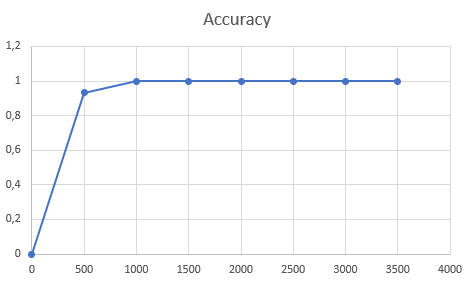
\includegraphics[width=0.8\linewidth]{accuracy_T}
  \caption{Graph showing the accuracy values (500-step intervals) achieved by the trained QDN with an unknown map.}
  \label{fig:accuracy_T}
\end{figure}

\section{Conclusion}
This paper has illustrated the suitability of convolutional neural networks for the problem of emulating dynamic $Q$-learning search results in maze solving. It has shown that, given a static or dynamic state space and a semi-observable environment, this problem is tractable with a QDN.

\end{document}